        \subsubsection{effects}
        Enthält die verwendeten Effekte die später zu unserer Szene hinzugefügt
        werden. Eine essenzielle Bedeutung kommt dabei den verschiedenen Partikeleffekten
        zu. \par
        \begin{figure}[htbp]
            \centering
            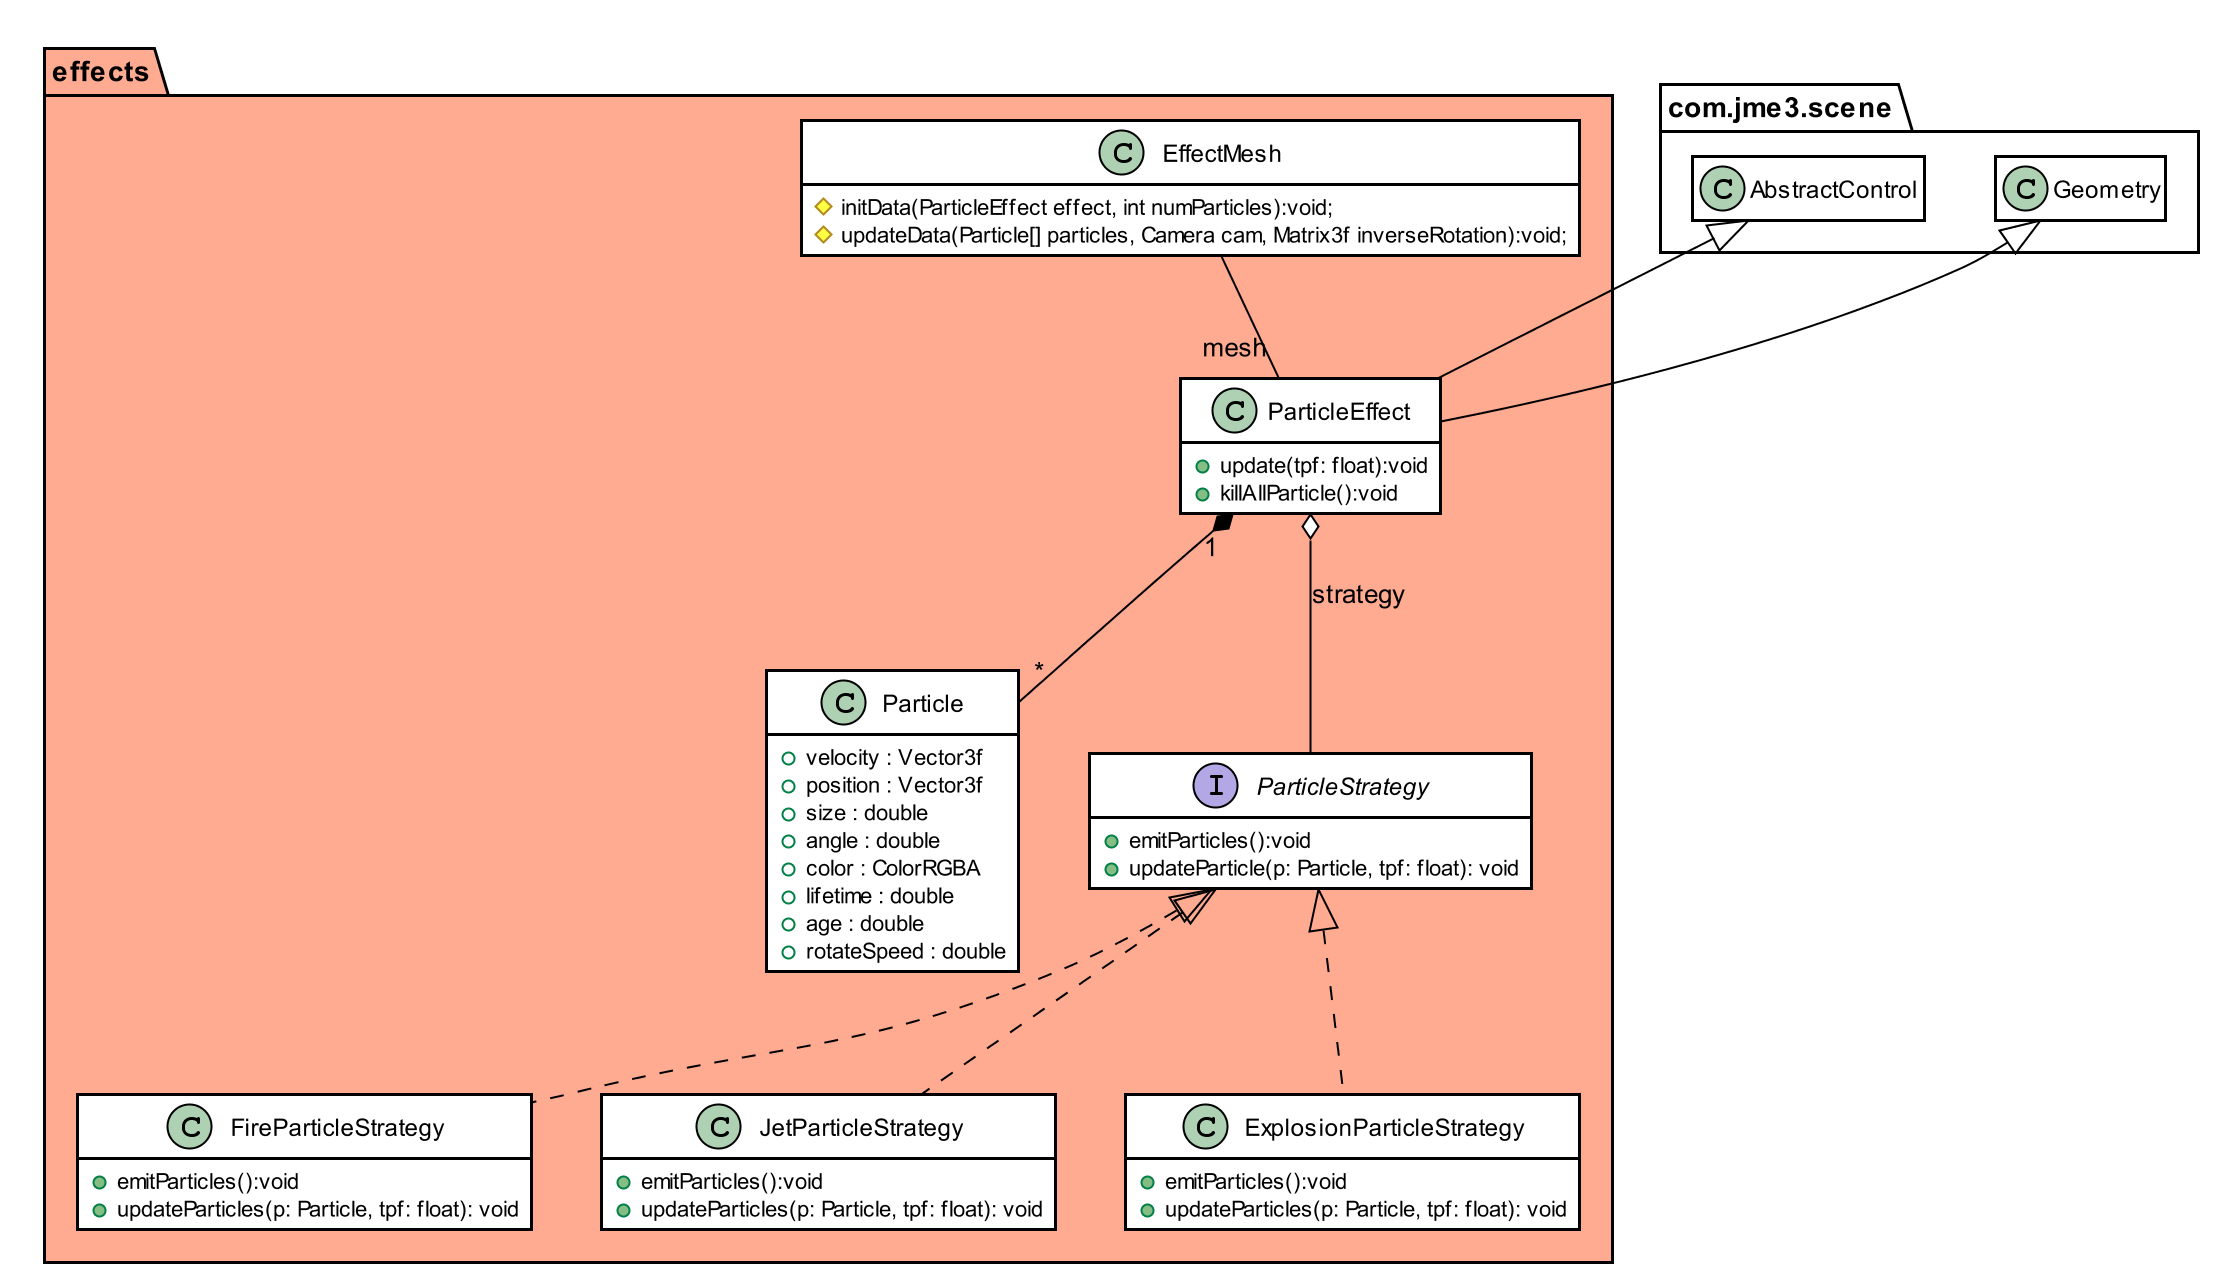
\includegraphics[width=1\linewidth]{InGameGrafik/Bilder/particleeffect.png}
            \caption{Klassendiagramm effects}
        \end{figure}
            \paragraph{\underline{Particle}} \mbox{}\\
                Repräsentiert die abstrakte Beschreibung eines einzelnen Partikels.
                Alle zur weiteren Berechnung wichtigen Informationen des Partikels für den 
                Partikeleffekt sind hierin festgehalten. \par
                \textbf{Attribute}
                \begin{itemize}
                    \item \textit{velocity}
                        \begin{leftbar}[0.9\linewidth]
                        Richtungsvektor unserer Partikels in der dreidimensionalen Szene.   
                        \end{leftbar}
                    \item \textit{position}
                        \begin{leftbar}[0.9\linewidth]
                        Positionsvektor unseres Partikels in der Szene; Angegeben für den Objektsraum.
                        \end{leftbar}
                    \pagebreak
                    \item \textit{size}
                        \begin{leftbar}[0.9\linewidth]
                        Beschreibt aktuelle Größe des Partikels.   
                        \end{leftbar}
                    \item \textit{angle}
                        \begin{leftbar}[0.9\linewidth]
                        Ausrichtung des Partikels in der Szene.   
                        \end{leftbar}    
                    \item \textit{color}
                        \begin{leftbar}[0.9\linewidth]
                        Aktuelle Farbe des Partikels in der Szene.  
                        \end{leftbar}
                    \item \textit{lifetime}
                        \begin{leftbar}[0.9\linewidth]
                        Beschreibt die Lebenszeit des Partikels in der Szene. Also wie lange sich
                        er bewegt bevor er an Ausgangspunkt gesetzt wird.   
                        \end{leftbar}
                    \item \textit{age}
                        \begin{leftbar}[0.9\linewidth]
                        Aktuelles Alter des Partikels, also vergangene Schritte seit emittieren.   
                        \end{leftbar}
                    \item \textit{rotateSpeed}
                        \begin{leftbar}[0.9\linewidth]
                        Beschreibt wie schnell sich der Partikel um seine eigene Achse dreht.  
                        \end{leftbar}
                \end{itemize}

                \paragraph{\underline{ParticleEffect}}\mbox{}\\
                    Eine Art Geometry im Kontext der JMonkeyEngine. So kann der Effect später einfach
                    zu seinem korrespndierenden Objekt in den Scenegraph hinzugefügt werden.
                    Zu einem ParticleEffect gehört immer eine entsprechende Anzahl von Partikeln.
                    \par

                    \textbf{Methoden}
                    \begin{itemize}
                        \item \textit{update(float tpf): void}
                            \begin{leftbar}[0.9\linewidth]
                            Aktualisiert den Partikeleffekt anhand der Strategy, sowie der framerate.  \\ 
                            \textbf{@param tpf} Times per frame.\\
                            \end{leftbar}
                        \item \textit{killAllParticle():void}
                            \begin{leftbar}[0.9\linewidth]
                            Lässt den Partikeleffekt wieder verschwinden.  
                            \end{leftbar}
                    \end{itemize}

                \pagebreak
                \paragraph{\underline{JetParticleStrategy}}\mbox{}\\
                    Beschreibt die genaue Strategie anhand der Partikel an einer Düse
                    emittiert werden.\par

                    \textbf{Methoden}
                    \begin{itemize}
                        \item \textit{emitParticles():void}
                            \begin{leftbar}[0.9\linewidth]
                            Emittiert einen einzigen Partikel nach "unten" in einem schmalen 
                            zufälligen Kegelradius .  
                            \end{leftbar}
                        \item \textit{updateParticles(Particle p, float tpf): void}
                            \begin{leftbar}[0.9\linewidth]
                            Aktualisiert die Partikel damit sie wie Düsenpartikel aussehen.\\  
                            \textbf{@param p} Der aktuelle Partikel der aktualisiert werden soll.\\
                            \textbf{@param tpf} Dime per frame.\\
                            \end{leftbar}
                    \end{itemize}
                
                \paragraph{\underline{FireParticleStrategy}}\mbox{}\\
                    Beschreibt die Strategie für Partikel von Feuer. Sie sollen ihre Farbe ändern
                    und sich von einem zentralen Punkt von Innen nach Außen bewegen.\par

                    \textbf{Methoden}
                    \begin{itemize}
                        \item \textit{emitParticles():void}
                            \begin{leftbar}[0.9\linewidth]
                            Wie ein einzelnes Feuerpartikel emittiert werden soll; zuälliger Winkel über
                            360 Grad mit sich ändernder Größe.   
                            \end{leftbar}
                        \item \textit{updateParticles(Particle p, float tpf): void}
                            \begin{leftbar}[0.9\linewidth]
                            Verändert die Attribute eines Feuerpartikels regelmäßig(abhängig von framerate).\\
                            \textbf{@param p} Der aktuelle Partikel der aktualisiert werden soll.\\
                            \textbf{@param tpf} Time per frame.\\
                            \end{leftbar}
                    \end{itemize}

                \pagebreak
                \paragraph{\underline{ExplosionParticleStrategy}}\mbox{}\\
                    Ist die Strategie wie ein PartikelEffekt für eine Explosion gesteuert
                    werden soll. \par

                    \textbf{Methoden}
                    \begin{itemize}
                        \item \textit{emitParticles():void}
                            \begin{leftbar}[0.9\linewidth]
                            Ein einzelner Explosionspartikel soll auf bestimmter Art und Weise emittiert werden
                            von einem Punkt aus in alle Richtungen.\\   
                            \end{leftbar}
                        \item \textit{updateParticles(Particle p, float tpf): void}
                            \begin{leftbar}[0.9\linewidth]
                            Aktualisiert die Attribute eines einzigen Partikels um eine Explosion zu sehen.
                            So wird die Geschwindigkeit, Position, Farbe etc. verändert.\\    
                            \textbf{@param p} Der aktuelle Partikel der aktualisiert werden soll.\\
                            \textbf{@param tpf} Time per frame.\\
                            \end{leftbar}
                    \end{itemize}
        \pagebreak